\cotefile{37}
\scanpage{52}
\noindent SGA 5 \(\overline{\underline{\mathrm{VII}}}\)\quad th de Lefschetz faible sans \unsure{supposer} \(X\) ni \(Y\) lisses (seulement \(X-Y\) lisse \ldots)

\noindent SGA 5 \(\overline{\underline{\unsure{\mathrm{V}|\mathrm{VI}}}}\)\quad \(\mathbb{Q}_{\ell}\)-faisceau : signaler définition raisonnable en termes de \uline{champ} \uline{associé}

% The replacement VI is below the cancelled numeral, within an open U-shaped curve.
\noindent SGA 5. \tikz[baseline=(old.base),x=1cm,y=1cm]{
\node[inner sep=0pt] (old) at (0,.44) {\(\deleted{\overline{\underline{\unsure{\mathrm{IV}|\mathrm{V}|\mathrm{VI}}}}}\)};
\node[inner sep=0pt] (vi) at (0,-.16) {\inserted{\(\overline{\underline{\mathrm{VI}}}\)}};
\draw[thin] (-.39,.06) .. controls (-.45,-.70) and (.42,-.73) .. (.76,.49);
}\quad Reprendre en langage de \(\mathbb{Z}_{\ell}\)-faisceaux ou\textsuperscript{\inserted{\unsure{*|+}}} \(\mathbb{Q}_{\ell}\)-faisceaux les notions essentielles dont il a été question dans SGA 4 (, Ajouter nouveau N\textsuperscript{\uline{o}}).

\noindent SGA 5 \(\overline{\underline{\mathrm{IV}}}\)\quad Essayer de faire dans le cas relativement lisse ttes les constructions essentielles

\figure{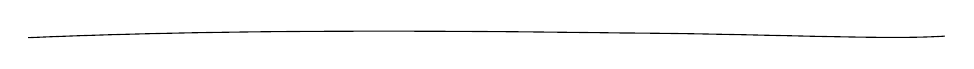
\begin{tikzpicture}[x=\linewidth,y=1cm]
\draw[thin] (0,0) .. controls (.23,.12) and (.49,.08) .. (.62,.06)
 .. controls (.77,.05) and (.90,-.03) .. (.96,.02);
\end{tikzpicture}}

\noindent \(\overline{\underline{\mathrm{VI}}}\)\quad \unsure{Systèmes|Système} projectifs \inserted{\tikz[baseline=(adiques.base)]{
\node[inner sep=0pt] (adiques) {adiques};
\draw[thin] ([xshift=-.35em,yshift=-1.2ex]adiques.south west)
 .. controls +(90:1.6ex) and +(-1em,-.2ex) .. (adiques.south)
 .. controls +(1.8em,.2ex) and +(0em,-1.1ex) .. ([xshift=1.1em,yshift=.3ex]adiques.east);
}} dans les catégories \unsure{dérivées} \ldots\ (ou dans thèse)

% Two faint isolated traces below the parenthesis; no lexical identity is assigned.
\figure{\begin{tikzpicture}[x=\linewidth,y=1cm]
\path[use as bounding box] (0,-.45) rectangle (1,.35);
\node[anchor=west,inner sep=0pt] at (.35,.08) {\unsure{\tikz[baseline=-.5ex,x=1cm,y=1cm]{\draw[thin,gray] (0,0) -- (.09,.04) -- (.17,-.01) -- (.19,.10) -- (.23,.16) -- (.27,.21); \draw[thin,gray] (.23,.16) -- (.21,.20);}}};
\node[anchor=west,inner sep=0pt] at (.45,-.18) {\unsure{\tikz[baseline=-.5ex,x=1cm,y=1cm]{\draw[thin,gray] (.08,.24) .. controls (.07,.19) and (.08,.15) .. (.08,.11) -- (.02,.15) -- (0,.08); \draw[thin,gray] (.08,.11) -- (.15,.02); \draw[thin,gray] (.03,-.04) -- (.08,-.10) -- (.14,-.04); \fill[gray] (.08,-.14) circle (.015);}}};
\end{tikzpicture}}
% slanted: a detached pair of dots, possibly incidental rather than a colon
\margin{\unsure{\tikz[baseline=-.3ex]{\fill (0,0) circle[radius=.35pt];\fill (.07,.10) circle[radius=.35pt];}}}

\noindent SGA 5 \(\mathrm{V}\)\quad dans introduction du \unsure{livre|Hom} ou de l'expo\unsure{sé} signaler l'ennui des coeff. trop particuliers \((\mathbb{Z}_{\ell},\,\unsure{\mathbb{Z}|Z}/\ell^{\unsure{\nu|n|N}}\mathbb{Z}\ -\,-)\)

\figure{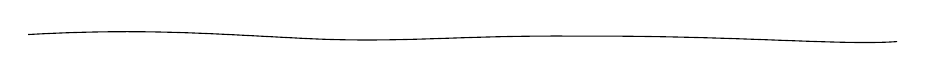
\begin{tikzpicture}[x=\linewidth,y=1cm]
\draw[thin] (0,.03) .. controls (.12,.11) and (.19,.04) .. (.29,-.02)
 .. controls (.39,-.08) and (.45,.02) .. (.57,.01)
 .. controls (.74,.02) and (.85,-.11) .. (.91,-.06);
\end{tikzpicture}}

\noindent \(\mathrm{I}\)\quad \S\ 5\qquad Donner, si \(i\unsure{{<}|{:}|{\in}}\unsure{\eta|y}\overset{\unsure{\sim}}{\longrightarrow} X\) inclusion du p\textsuperscript{t} générique, et \(F_{\eta}\) Module loc. \unsure{libre} sur \(\eta\)
\[
 D\bigl(i_{*}(F_{\eta})\bigr)=i_{*}\bigl(D(F_{\eta})\bigr)
\]
% archive sheet number: 51
\clearpage
